\PassOptionsToPackage{unicode=true}{hyperref} % options for packages loaded elsewhere
\PassOptionsToPackage{hyphens}{url}
\PassOptionsToPackage{dvipsnames,svgnames*,x11names*}{xcolor}
%
\documentclass[paper=a4,justified,a4paper]{tufte-handout}
\usepackage{lmodern}
\usepackage{amssymb,amsmath}
\usepackage{ifxetex,ifluatex}
\usepackage{fixltx2e} % provides \textsubscript
\ifnum 0\ifxetex 1\fi\ifluatex 1\fi=0 % if pdftex
  \usepackage[T1]{fontenc}
  \usepackage[utf8]{inputenc}
  \usepackage{textcomp} % provides euro and other symbols
\else % if luatex or xelatex
  \usepackage{unicode-math}
  \defaultfontfeatures{Ligatures=TeX,Scale=MatchLowercase}
\fi
% use upquote if available, for straight quotes in verbatim environments
\IfFileExists{upquote.sty}{\usepackage{upquote}}{}
% use microtype if available
\IfFileExists{microtype.sty}{%
\usepackage[]{microtype}
\UseMicrotypeSet[protrusion]{basicmath} % disable protrusion for tt fonts
}{}
\IfFileExists{parskip.sty}{%
\usepackage{parskip}
}{% else
\setlength{\parindent}{0pt}
\setlength{\parskip}{6pt plus 2pt minus 1pt}
}
\usepackage{xcolor}
\usepackage{hyperref}
\hypersetup{
            pdftitle={Assignment 6 Working Methods - Initial Reflection Report},
            pdfauthor={Helena Rasche},
            colorlinks=true,
            linkcolor=Maroon,
            filecolor=Maroon,
            citecolor=Blue,
            urlcolor=Blue,
            breaklinks=true}
\urlstyle{same}  % don't use monospace font for urls
\usepackage{longtable,booktabs}
% Fix footnotes in tables (requires footnote package)
\IfFileExists{footnote.sty}{\usepackage{footnote}\makesavenoteenv{longtable}}{}
\usepackage{graphicx,grffile}
\makeatletter
\def\maxwidth{\ifdim\Gin@nat@width>\linewidth\linewidth\else\Gin@nat@width\fi}
\def\maxheight{\ifdim\Gin@nat@height>\textheight\textheight\else\Gin@nat@height\fi}
\makeatother
% Scale images if necessary, so that they will not overflow the page
% margins by default, and it is still possible to overwrite the defaults
% using explicit options in \includegraphics[width, height, ...]{}
\setkeys{Gin}{width=\maxwidth,height=\maxheight,keepaspectratio}
\setlength{\emergencystretch}{3em}  % prevent overfull lines
\providecommand{\tightlist}{%
  \setlength{\itemsep}{0pt}\setlength{\parskip}{0pt}}
\setcounter{secnumdepth}{0}
% Redefines (sub)paragraphs to behave more like sections
\ifx\paragraph\undefined\else
\let\oldparagraph\paragraph
\renewcommand{\paragraph}[1]{\oldparagraph{#1}\mbox{}}
\fi
\ifx\subparagraph\undefined\else
\let\oldsubparagraph\subparagraph
\renewcommand{\subparagraph}[1]{\oldsubparagraph{#1}\mbox{}}
\fi

% set default figure placement to htbp
\makeatletter
\def\fps@figure{htbp}
\makeatother

\usepackage{pdfpages}

%%%%%%%%%%% Header and Footer %%%%%%%%%%%%%%%%%%
\fancyfoot[CE,CO]{\flushright 
\includegraphics[width=3cm]{../avans.jpg}}
\fancyhead[CE,CO]{\flushleft \smallcaps{\today}}

\usepackage[]{natbib}
\bibliographystyle{plainnat}

\title{Assignment 6 Working Methods - Initial Reflection Report}
\author{Helena Rasche}
\date{2022-02-07}

\begin{document}
\maketitle
\begin{abstract}
Given the previously sub-optimal Python lesson which relied on students
individually completing assignments, a task with which they struggled
and felt quite isolated, here we discuss the replacement of individual
exercises with pair programming. This improved the lesson significantly,
with the additional improvement of teaching an industry-relevant skill;
pair programming is often used in the industry to decrease defects and
improve the onboarding process.
\end{abstract}
\noindent\rule{5in}{0.4pt}


\hypertarget{pair-programming}{%
\section{Pair Programming}\label{pair-programming}}

Pair programming is a software development methodology requiring two
programmers to work together to solve problems and implement code.

\begin{quote}
One, the driver, writes code while the other, the observer or navigator,
reviews each line of code as it is typed in. The two programmers switch
roles frequently \citep{Williams}
\end{quote}

\begin{figure}
\centering
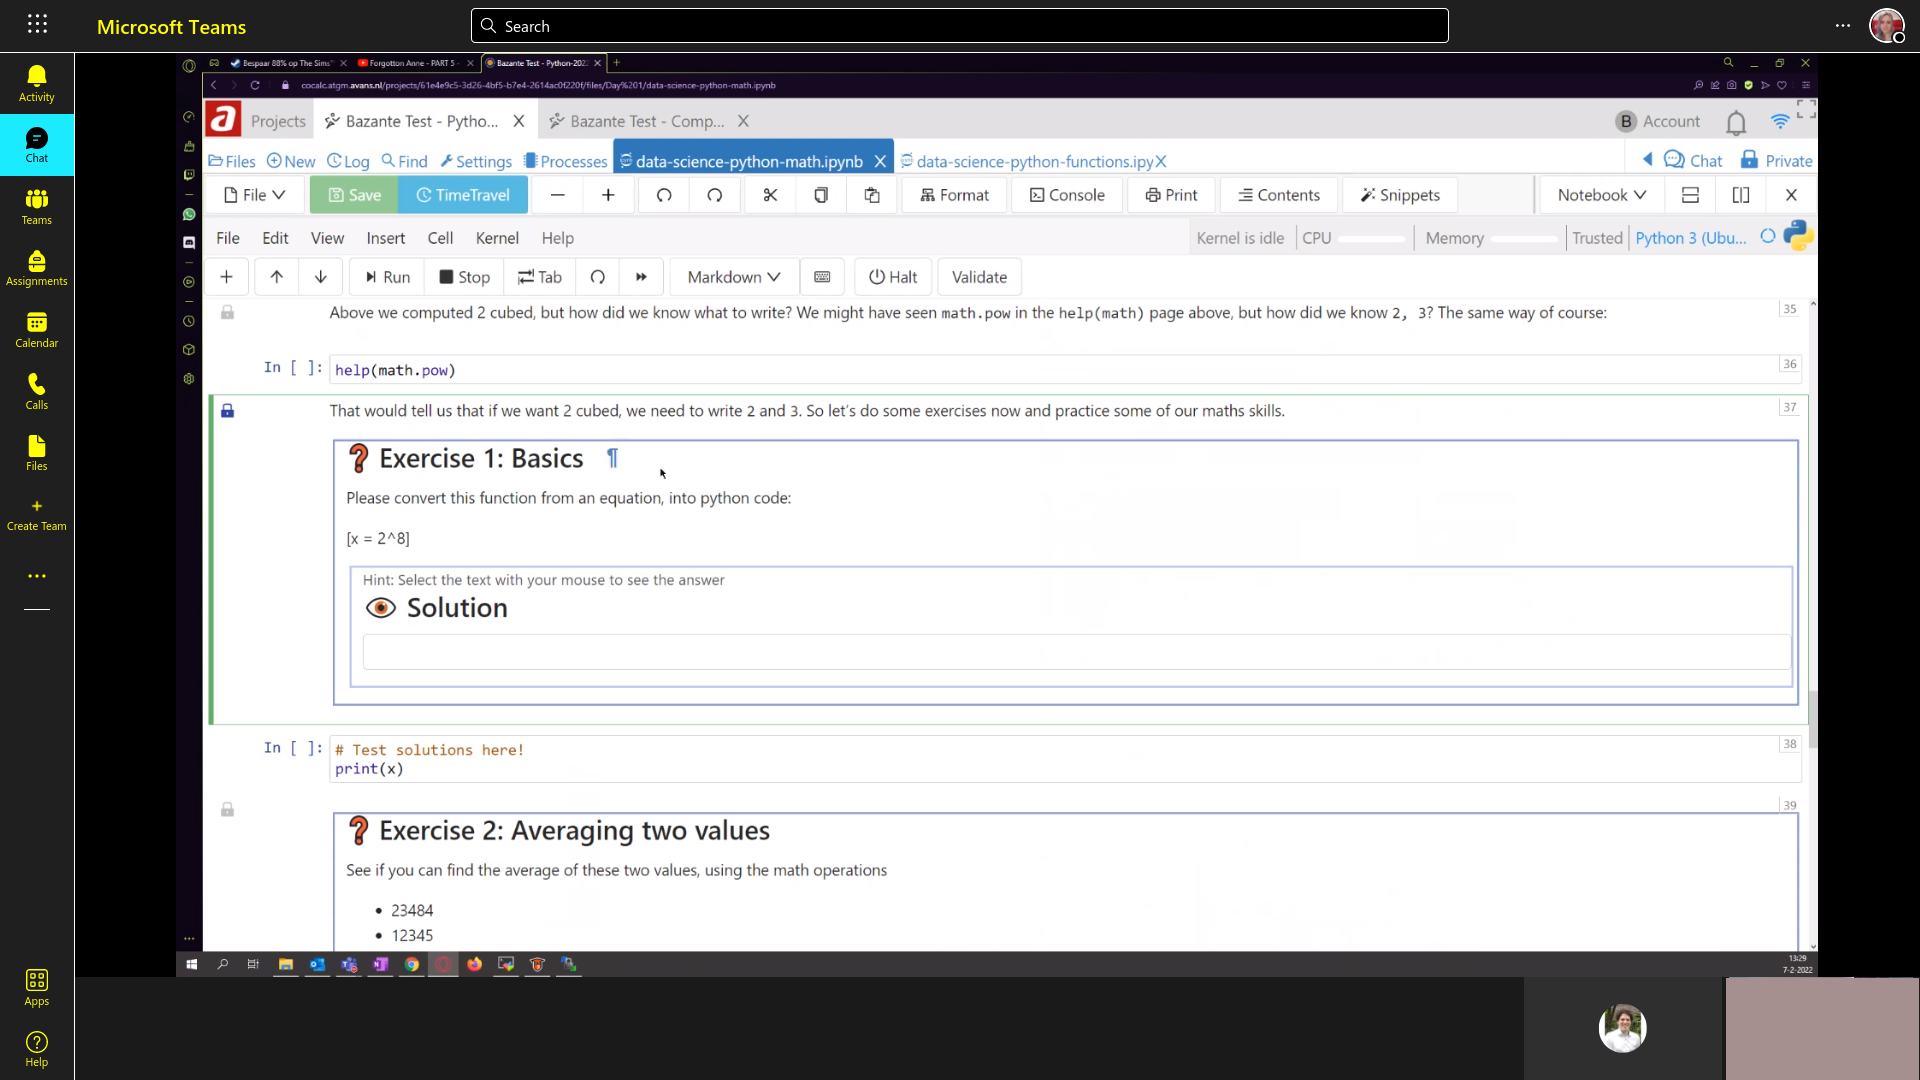
\includegraphics{sharing.png}
\caption{Screenshot of a teams call in which two students sit, one
actively working on writing code, the other leading the discussion. One
student's screen is showing CoCalc, a notebook platform where students
can type code and immediately evaluate it's correctness. This platform
allows us to write rich documentation, provide links to external
resources, and write exercise problems which students can then easily
work on individually or together.}
\end{figure}

Here we adapt this to the teaching environment via use of breakout rooms
with two students, and screen sharing permitting the same situation of a
``driver'' and a ``navigator''. This should reduce cognitive load and
frustration amongst students and allow them to rely on each other more
for technical discussions, rather than seeing the teacher as the primary
source of information \citep{Williams_2001}.

\hypertarget{positives}{%
\subsection{Positives}\label{positives}}

This methodology should hopefully bring significant improvements for
students as it has been empirically shown to be an effective learning
methodology for students
\citep{mendes2005investigating, mendes2006replicated}. Specifically this
technique has also been shown to be extremely beneficial for women in
computer science and gives them better chances for success in future
programming endeavours \citep{werner2004pair}, potentially by changing
the concept of programming from a solo activity to a collaborative
activity as it often exists in practice. Given that in business and
academia, programming often involves peer code review to ensure high
quality results, this makes it an ideal fit for our educational
practices and a very positive experimental change to make to classes.

\hypertarget{pitfalls}{%
\subsection{Pitfalls}\label{pitfalls}}

However there are some notable pair programming pitfalls in a teaching
environment, such as the student with more coding experience doing all
of the work by themselves
\citep{cliburn2003experiences, Williams_2002, mcdowell2003experimenting},
or students failing to swap roles leading to a similar result. These
issues can be mitigated through a number of methods including student
self-reporting their contributions or lecturers taking a supervisory
role \citep{Williams_2002}. \citet{Mentz_2008} additionally reports
success with the integration of the concepts of ``Cooperative Learning''
and provides guidelines for mitigating potential failure modes. These
can be addressed easily via teacher intervention and were done so during
the course, limited only by the availability of teacher and/or TOAs
moving between groups.

\hypertarget{feedback}{%
\subsection{Feedback}\label{feedback}}

Student feedback was extremely positive, averaging 4.35 for all
measures. The students overall liked the use of pair programming in
their learning environment and found that it invited them to actively
participate in the lesson.

\begin{longtable}[]{@{}lllllll@{}}
\toprule
\begin{minipage}[b]{0.18\columnwidth}\raggedright
Question\strut
\end{minipage} & \begin{minipage}[b]{0.07\columnwidth}\raggedright
Min\strut
\end{minipage} & \begin{minipage}[b]{0.07\columnwidth}\raggedright
Max\strut
\end{minipage} & \begin{minipage}[b]{0.09\columnwidth}\raggedright
Mean\strut
\end{minipage} & \begin{minipage}[b]{0.18\columnwidth}\raggedright
Std.Dev.\strut
\end{minipage} & \begin{minipage}[b]{0.13\columnwidth}\raggedright
Median\strut
\end{minipage} & \begin{minipage}[b]{0.09\columnwidth}\raggedright
Mode\strut
\end{minipage}\tabularnewline
\midrule
\endhead
\begin{minipage}[t]{0.18\columnwidth}\raggedright
\scriptsize The teaching method(s) used in the lesson fit the content of
the lesson.\strut
\end{minipage} & \begin{minipage}[t]{0.07\columnwidth}\raggedright
4\strut
\end{minipage} & \begin{minipage}[t]{0.07\columnwidth}\raggedright
5\strut
\end{minipage} & \begin{minipage}[t]{0.09\columnwidth}\raggedright
4.41\strut
\end{minipage} & \begin{minipage}[t]{0.18\columnwidth}\raggedright
0.49\strut
\end{minipage} & \begin{minipage}[t]{0.13\columnwidth}\raggedright
4\strut
\end{minipage} & \begin{minipage}[t]{0.09\columnwidth}\raggedright
4\strut
\end{minipage}\tabularnewline
\begin{minipage}[t]{0.18\columnwidth}\raggedright
\scriptsize I liked the teaching method(s) used in the lesson.\strut
\end{minipage} & \begin{minipage}[t]{0.07\columnwidth}\raggedright
3\strut
\end{minipage} & \begin{minipage}[t]{0.07\columnwidth}\raggedright
5\strut
\end{minipage} & \begin{minipage}[t]{0.09\columnwidth}\raggedright
4.33\strut
\end{minipage} & \begin{minipage}[t]{0.18\columnwidth}\raggedright
0.62\strut
\end{minipage} & \begin{minipage}[t]{0.13\columnwidth}\raggedright
4\strut
\end{minipage} & \begin{minipage}[t]{0.09\columnwidth}\raggedright
4\strut
\end{minipage}\tabularnewline
\begin{minipage}[t]{0.18\columnwidth}\raggedright
\scriptsize The teacher's instruction was clear to me.\strut
\end{minipage} & \begin{minipage}[t]{0.07\columnwidth}\raggedright
4\strut
\end{minipage} & \begin{minipage}[t]{0.07\columnwidth}\raggedright
5\strut
\end{minipage} & \begin{minipage}[t]{0.09\columnwidth}\raggedright
4.33\strut
\end{minipage} & \begin{minipage}[t]{0.18\columnwidth}\raggedright
0.47\strut
\end{minipage} & \begin{minipage}[t]{0.13\columnwidth}\raggedright
4\strut
\end{minipage} & \begin{minipage}[t]{0.09\columnwidth}\raggedright
4\strut
\end{minipage}\tabularnewline
\begin{minipage}[t]{0.18\columnwidth}\raggedright
\scriptsize The used teaching methods invited me to active
participation.\strut
\end{minipage} & \begin{minipage}[t]{0.07\columnwidth}\raggedright
4\strut
\end{minipage} & \begin{minipage}[t]{0.07\columnwidth}\raggedright
5\strut
\end{minipage} & \begin{minipage}[t]{0.09\columnwidth}\raggedright
4.41\strut
\end{minipage} & \begin{minipage}[t]{0.18\columnwidth}\raggedright
0.49\strut
\end{minipage} & \begin{minipage}[t]{0.13\columnwidth}\raggedright
4\strut
\end{minipage} & \begin{minipage}[t]{0.09\columnwidth}\raggedright
4\strut
\end{minipage}\tabularnewline
\begin{minipage}[t]{0.18\columnwidth}\raggedright
\scriptsize The teaching methods used fit my way of learning.\strut
\end{minipage} & \begin{minipage}[t]{0.07\columnwidth}\raggedright
3\strut
\end{minipage} & \begin{minipage}[t]{0.07\columnwidth}\raggedright
5\strut
\end{minipage} & \begin{minipage}[t]{0.09\columnwidth}\raggedright
4.33\strut
\end{minipage} & \begin{minipage}[t]{0.18\columnwidth}\raggedright
0.62\strut
\end{minipage} & \begin{minipage}[t]{0.13\columnwidth}\raggedright
4\strut
\end{minipage} & \begin{minipage}[t]{0.09\columnwidth}\raggedright
4\strut
\end{minipage}\tabularnewline
\begin{minipage}[t]{0.18\columnwidth}\raggedright
\scriptsize I liked the teacher's approach in this lesson better than in
other lessons.\strut
\end{minipage} & \begin{minipage}[t]{0.07\columnwidth}\raggedright
3\strut
\end{minipage} & \begin{minipage}[t]{0.07\columnwidth}\raggedright
5\strut
\end{minipage} & \begin{minipage}[t]{0.09\columnwidth}\raggedright
3.91\strut
\end{minipage} & \begin{minipage}[t]{0.18\columnwidth}\raggedright
0.49\strut
\end{minipage} & \begin{minipage}[t]{0.13\columnwidth}\raggedright
4\strut
\end{minipage} & \begin{minipage}[t]{0.09\columnwidth}\raggedright
4\strut
\end{minipage}\tabularnewline
\begin{minipage}[t]{0.18\columnwidth}\raggedright
\scriptsize I thought it was a nice lesson.\strut
\end{minipage} & \begin{minipage}[t]{0.07\columnwidth}\raggedright
4\strut
\end{minipage} & \begin{minipage}[t]{0.07\columnwidth}\raggedright
5\strut
\end{minipage} & \begin{minipage}[t]{0.09\columnwidth}\raggedright
4.75\strut
\end{minipage} & \begin{minipage}[t]{0.18\columnwidth}\raggedright
0.43\strut
\end{minipage} & \begin{minipage}[t]{0.13\columnwidth}\raggedright
5\strut
\end{minipage} & \begin{minipage}[t]{0.09\columnwidth}\raggedright
5\strut
\end{minipage}\tabularnewline
\bottomrule
\end{longtable}

They additionally provided comments on the above, filtered for
comments\footnote{The full response set is attached at the end.}
specifically concerning the aspect of pair programming:

\begin{itemize}
\tightlist
\item
  \small ``The breakout rooms are very nice. It is a nice way to work
  with the students and get some interaction and get to work with the
  theory. For me the theory stick better.''
\item
  \small ``It was a lot of information for one day but working on the
  excercises together helped a lot''
\item
  \small ``I think working in pairs in breakoutrooms really helped in
  solving some of the questions and getting some insight''
\item
  \small ``I think it was nice to work on it together in breakout rooms,
  {[}\ldots{}{]}''
\item
  \small ``The alternation between explanations and making assignments
  was good.''
\item
  \small ``Good mix between excersises and theory''
\end{itemize}

Given the feedback it can be concluded that this was a successful
intervention and practice that should be continued throughout the rest
of the period. Additionally given that there are two sections of this
course, one taught by a teacher not employing this method, it will
provide an opportunity to further confirm or refute the success of the
experiment.

\hypertarget{reflection}{%
\section{Reflection}\label{reflection}}

In this lesson a significant overhaul was made to the material to
function better as an online lesson. Further an intervention of pair
programming was applied via breakout rooms and pairing students off in
duos. I decided in the first breakout room to give students some privacy
and let them discuss together, while in the second round of breakout
rooms I ``walked around'' and visited the various breakout rooms to see
how students were getting on\footnote{This proved to be quite useful, I
  could see students making mistakes I would not have noticed otherwise,
  or if I'd only seen the final result.}. The breakout rooms went
successfully and students shared their results at the end. This is a
process I wish to automate in the future, sharing results back, in order
to give students some anonymity while I discuss common issues I saw
during their exercise. Here I could only comment on mistakes based on
their final result (if I did not observe) or the process if I was
present in the breakout room to see the specific error occur.

\hypertarget{looking-back}{%
\subsection{Looking Back}\label{looking-back}}

Overall this went quite well, I saw students interacting well and
switching off between roles but could not confirm the uniformity of
switching each time. I think this was a very successful intervention
based on my observations as a teacher and the reporting of the students.

\hypertarget{awareness}{%
\subsection{Awareness}\label{awareness}}

Based on the research included here, I think I need to further improve
my observation of the students, either transparently via the programming
environment we're using, or directly via my presence in the breakout
rooms. One of these options scales better, but it might leave students
without a good source of advice when they encounter difficulties in the
exercises. Whether this builds skills to overcome small challenges, or
leaves them struggling when they need assistance is yet to be seen.

\hypertarget{alternatives}{%
\subsection{Alternatives}\label{alternatives}}

Instead of pairing them in duos, I could try pairing them in threes but
this might lead to one person sitting back and not participating,
whereas the pair situation forces them to participate but doesn't risk
them feeling isolated. Next time I should continue my experiments of
whether or not to visit them in their individual breakout rooms during
the exercises to examine what effects that has on students, and
additionally survey them on their preferences to find a common solution
that achieves both my goals of a more supportive learning environment
while avoiding disrupting them or having them feel a stressful scenario
where they pressured to defend a topic they do not know well.

\hypertarget{trials}{%
\subsection{Trials}\label{trials}}

Given the results of \citet{werner2004pair} I'll be carefully watching
the outcomes of my course compared to my colleague's to see how the
women in my class feel compared to theirs, and if the difference is
significant to help them implement pair programming in their class.
However I need to be careful that I'm not blinded by the success of this
methodology on a global scale, and make sure I am adapting to students
who struggle with this model and prefer working on their own, perhaps to
be determined via further student surveying.

\hypertarget{supplemental-data}{%
\section{Supplemental Data}\label{supplemental-data}}

\begin{longtable}[]{@{}lllllllllllll@{}}
\toprule
\begin{minipage}[b]{0.07\columnwidth}\raggedright
ID\strut
\end{minipage} & \begin{minipage}[b]{0.04\columnwidth}\raggedright
2\strut
\end{minipage} & \begin{minipage}[b]{0.04\columnwidth}\raggedright
3\strut
\end{minipage} & \begin{minipage}[b]{0.04\columnwidth}\raggedright
4\strut
\end{minipage} & \begin{minipage}[b]{0.04\columnwidth}\raggedright
5\strut
\end{minipage} & \begin{minipage}[b]{0.04\columnwidth}\raggedright
6\strut
\end{minipage} & \begin{minipage}[b]{0.04\columnwidth}\raggedright
7\strut
\end{minipage} & \begin{minipage}[b]{0.04\columnwidth}\raggedright
8\strut
\end{minipage} & \begin{minipage}[b]{0.04\columnwidth}\raggedright
9\strut
\end{minipage} & \begin{minipage}[b]{0.07\columnwidth}\raggedright
10\strut
\end{minipage} & \begin{minipage}[b]{0.07\columnwidth}\raggedright
11\strut
\end{minipage} & \begin{minipage}[b]{0.07\columnwidth}\raggedright
12\strut
\end{minipage} & \begin{minipage}[b]{0.07\columnwidth}\raggedright
13\strut
\end{minipage}\tabularnewline
\midrule
\endhead
\begin{minipage}[t]{0.07\columnwidth}\raggedright
\scriptsize The teaching method (s) used in the lesson fit the content
of the lesson.\strut
\end{minipage} & \begin{minipage}[t]{0.04\columnwidth}\raggedright
5\strut
\end{minipage} & \begin{minipage}[t]{0.04\columnwidth}\raggedright
5\strut
\end{minipage} & \begin{minipage}[t]{0.04\columnwidth}\raggedright
4\strut
\end{minipage} & \begin{minipage}[t]{0.04\columnwidth}\raggedright
4\strut
\end{minipage} & \begin{minipage}[t]{0.04\columnwidth}\raggedright
5\strut
\end{minipage} & \begin{minipage}[t]{0.04\columnwidth}\raggedright
4\strut
\end{minipage} & \begin{minipage}[t]{0.04\columnwidth}\raggedright
5\strut
\end{minipage} & \begin{minipage}[t]{0.04\columnwidth}\raggedright
4\strut
\end{minipage} & \begin{minipage}[t]{0.07\columnwidth}\raggedright
4\strut
\end{minipage} & \begin{minipage}[t]{0.07\columnwidth}\raggedright
4\strut
\end{minipage} & \begin{minipage}[t]{0.07\columnwidth}\raggedright
5\strut
\end{minipage} & \begin{minipage}[t]{0.07\columnwidth}\raggedright
4\strut
\end{minipage}\tabularnewline
\begin{minipage}[t]{0.07\columnwidth}\raggedright
\scriptsize I liked the teaching method (s) used in the lesson.\strut
\end{minipage} & \begin{minipage}[t]{0.04\columnwidth}\raggedright
5\strut
\end{minipage} & \begin{minipage}[t]{0.04\columnwidth}\raggedright
4\strut
\end{minipage} & \begin{minipage}[t]{0.04\columnwidth}\raggedright
4\strut
\end{minipage} & \begin{minipage}[t]{0.04\columnwidth}\raggedright
5\strut
\end{minipage} & \begin{minipage}[t]{0.04\columnwidth}\raggedright
4\strut
\end{minipage} & \begin{minipage}[t]{0.04\columnwidth}\raggedright
5\strut
\end{minipage} & \begin{minipage}[t]{0.04\columnwidth}\raggedright
3\strut
\end{minipage} & \begin{minipage}[t]{0.04\columnwidth}\raggedright
5\strut
\end{minipage} & \begin{minipage}[t]{0.07\columnwidth}\raggedright
4\strut
\end{minipage} & \begin{minipage}[t]{0.07\columnwidth}\raggedright
4\strut
\end{minipage} & \begin{minipage}[t]{0.07\columnwidth}\raggedright
5\strut
\end{minipage} & \begin{minipage}[t]{0.07\columnwidth}\raggedright
4\strut
\end{minipage}\tabularnewline
\begin{minipage}[t]{0.07\columnwidth}\raggedright
\scriptsize The teacher's instruction was clear to me.\strut
\end{minipage} & \begin{minipage}[t]{0.04\columnwidth}\raggedright
4\strut
\end{minipage} & \begin{minipage}[t]{0.04\columnwidth}\raggedright
4\strut
\end{minipage} & \begin{minipage}[t]{0.04\columnwidth}\raggedright
5\strut
\end{minipage} & \begin{minipage}[t]{0.04\columnwidth}\raggedright
4\strut
\end{minipage} & \begin{minipage}[t]{0.04\columnwidth}\raggedright
4\strut
\end{minipage} & \begin{minipage}[t]{0.04\columnwidth}\raggedright
5\strut
\end{minipage} & \begin{minipage}[t]{0.04\columnwidth}\raggedright
4\strut
\end{minipage} & \begin{minipage}[t]{0.04\columnwidth}\raggedright
5\strut
\end{minipage} & \begin{minipage}[t]{0.07\columnwidth}\raggedright
4\strut
\end{minipage} & \begin{minipage}[t]{0.07\columnwidth}\raggedright
4\strut
\end{minipage} & \begin{minipage}[t]{0.07\columnwidth}\raggedright
4\strut
\end{minipage} & \begin{minipage}[t]{0.07\columnwidth}\raggedright
5\strut
\end{minipage}\tabularnewline
\begin{minipage}[t]{0.07\columnwidth}\raggedright
\scriptsize The used teaching methods invited me to active
participation.\strut
\end{minipage} & \begin{minipage}[t]{0.04\columnwidth}\raggedright
4\strut
\end{minipage} & \begin{minipage}[t]{0.04\columnwidth}\raggedright
5\strut
\end{minipage} & \begin{minipage}[t]{0.04\columnwidth}\raggedright
5\strut
\end{minipage} & \begin{minipage}[t]{0.04\columnwidth}\raggedright
5\strut
\end{minipage} & \begin{minipage}[t]{0.04\columnwidth}\raggedright
4\strut
\end{minipage} & \begin{minipage}[t]{0.04\columnwidth}\raggedright
5\strut
\end{minipage} & \begin{minipage}[t]{0.04\columnwidth}\raggedright
4\strut
\end{minipage} & \begin{minipage}[t]{0.04\columnwidth}\raggedright
5\strut
\end{minipage} & \begin{minipage}[t]{0.07\columnwidth}\raggedright
4\strut
\end{minipage} & \begin{minipage}[t]{0.07\columnwidth}\raggedright
4\strut
\end{minipage} & \begin{minipage}[t]{0.07\columnwidth}\raggedright
4\strut
\end{minipage} & \begin{minipage}[t]{0.07\columnwidth}\raggedright
4\strut
\end{minipage}\tabularnewline
\begin{minipage}[t]{0.07\columnwidth}\raggedright
\scriptsize The teaching methods used fit my way of learning.\strut
\end{minipage} & \begin{minipage}[t]{0.04\columnwidth}\raggedright
4\strut
\end{minipage} & \begin{minipage}[t]{0.04\columnwidth}\raggedright
4\strut
\end{minipage} & \begin{minipage}[t]{0.04\columnwidth}\raggedright
5\strut
\end{minipage} & \begin{minipage}[t]{0.04\columnwidth}\raggedright
4\strut
\end{minipage} & \begin{minipage}[t]{0.04\columnwidth}\raggedright
5\strut
\end{minipage} & \begin{minipage}[t]{0.04\columnwidth}\raggedright
5\strut
\end{minipage} & \begin{minipage}[t]{0.04\columnwidth}\raggedright
4\strut
\end{minipage} & \begin{minipage}[t]{0.04\columnwidth}\raggedright
5\strut
\end{minipage} & \begin{minipage}[t]{0.07\columnwidth}\raggedright
4\strut
\end{minipage} & \begin{minipage}[t]{0.07\columnwidth}\raggedright
4\strut
\end{minipage} & \begin{minipage}[t]{0.07\columnwidth}\raggedright
5\strut
\end{minipage} & \begin{minipage}[t]{0.07\columnwidth}\raggedright
3\strut
\end{minipage}\tabularnewline
\begin{minipage}[t]{0.07\columnwidth}\raggedright
\scriptsize I liked the teacher's approach in this lesson better than in
other lessons.\strut
\end{minipage} & \begin{minipage}[t]{0.04\columnwidth}\raggedright
4\strut
\end{minipage} & \begin{minipage}[t]{0.04\columnwidth}\raggedright
4\strut
\end{minipage} & \begin{minipage}[t]{0.04\columnwidth}\raggedright
4\strut
\end{minipage} & \begin{minipage}[t]{0.04\columnwidth}\raggedright
4\strut
\end{minipage} & \begin{minipage}[t]{0.04\columnwidth}\raggedright
4\strut
\end{minipage} & \begin{minipage}[t]{0.04\columnwidth}\raggedright
3\strut
\end{minipage} & \begin{minipage}[t]{0.04\columnwidth}\raggedright
4\strut
\end{minipage} & \begin{minipage}[t]{0.04\columnwidth}\raggedright
4\strut
\end{minipage} & \begin{minipage}[t]{0.07\columnwidth}\raggedright
4\strut
\end{minipage} & \begin{minipage}[t]{0.07\columnwidth}\raggedright
4\strut
\end{minipage} & \begin{minipage}[t]{0.07\columnwidth}\raggedright
5\strut
\end{minipage} & \begin{minipage}[t]{0.07\columnwidth}\raggedright
3\strut
\end{minipage}\tabularnewline
\begin{minipage}[t]{0.07\columnwidth}\raggedright
\scriptsize I thought it was a nice lesson.\strut
\end{minipage} & \begin{minipage}[t]{0.04\columnwidth}\raggedright
5\strut
\end{minipage} & \begin{minipage}[t]{0.04\columnwidth}\raggedright
5\strut
\end{minipage} & \begin{minipage}[t]{0.04\columnwidth}\raggedright
5\strut
\end{minipage} & \begin{minipage}[t]{0.04\columnwidth}\raggedright
5\strut
\end{minipage} & \begin{minipage}[t]{0.04\columnwidth}\raggedright
5\strut
\end{minipage} & \begin{minipage}[t]{0.04\columnwidth}\raggedright
4\strut
\end{minipage} & \begin{minipage}[t]{0.04\columnwidth}\raggedright
5\strut
\end{minipage} & \begin{minipage}[t]{0.04\columnwidth}\raggedright
5\strut
\end{minipage} & \begin{minipage}[t]{0.07\columnwidth}\raggedright
4\strut
\end{minipage} & \begin{minipage}[t]{0.07\columnwidth}\raggedright
4\strut
\end{minipage} & \begin{minipage}[t]{0.07\columnwidth}\raggedright
5\strut
\end{minipage} & \begin{minipage}[t]{0.07\columnwidth}\raggedright
5\strut
\end{minipage}\tabularnewline
\bottomrule
\end{longtable}

\begin{longtable}[]{@{}ll@{}}
\toprule
\begin{minipage}[b]{0.04\columnwidth}\raggedright
ID\strut
\end{minipage} & \begin{minipage}[b]{0.90\columnwidth}\raggedright
Remarks/Suggestions on any of the above points\strut
\end{minipage}\tabularnewline
\midrule
\endhead
\begin{minipage}[t]{0.04\columnwidth}\raggedright
2\strut
\end{minipage} & \begin{minipage}[t]{0.90\columnwidth}\raggedright
\scriptsize ``Helena does explain it clear and very well, albeit
sometimes a bit too quick''\strut
\end{minipage}\tabularnewline
\begin{minipage}[t]{0.04\columnwidth}\raggedright
6\strut
\end{minipage} & \begin{minipage}[t]{0.90\columnwidth}\raggedright
\scriptsize you're doing a great job. The breakout rooms are very nice.
It is a nice way to work with the students and get some interaction and
get to work with the theory. For me the theory stick better.\strut
\end{minipage}\tabularnewline
\begin{minipage}[t]{0.04\columnwidth}\raggedright
7\strut
\end{minipage} & \begin{minipage}[t]{0.90\columnwidth}\raggedright
\scriptsize ``great lesson, it was a lot of information for one day but
working on the excercises together helped a lot. bugs happen even to the
best so no complains :)''\strut
\end{minipage}\tabularnewline
\begin{minipage}[t]{0.04\columnwidth}\raggedright
8\strut
\end{minipage} & \begin{minipage}[t]{0.90\columnwidth}\raggedright
\scriptsize I think working in pairs in breakoutrooms really helped in
solving some of the questions and getting some insight\strut
\end{minipage}\tabularnewline
\begin{minipage}[t]{0.04\columnwidth}\raggedright
9\strut
\end{minipage} & \begin{minipage}[t]{0.90\columnwidth}\raggedright
\scriptsize ``I think it was nice to work on it together in breakout
rooms, sometimes it was bit to fast to follow every steps, but still
manageable. Also I really like how Helena approaches us and reacts when
we ask a question.''\strut
\end{minipage}\tabularnewline
\begin{minipage}[t]{0.04\columnwidth}\raggedright
10\strut
\end{minipage} & \begin{minipage}[t]{0.90\columnwidth}\raggedright
\scriptsize ``The explanation was clear. All the topics were clearly
covered. At times, it was perhaps a little too fast, which made it
difficult to follow. The alternation between explanations and making
assignments was good.''\strut
\end{minipage}\tabularnewline
\begin{minipage}[t]{0.04\columnwidth}\raggedright
11\strut
\end{minipage} & \begin{minipage}[t]{0.90\columnwidth}\raggedright
\scriptsize ``I liked the lesson, it was all still quite new so it was a
lot of information for today. It was nice that there was some
interaction so I could follow along with you to understand the process
more. The explanation was clear and easy to follow.''\strut
\end{minipage}\tabularnewline
\begin{minipage}[t]{0.04\columnwidth}\raggedright
12\strut
\end{minipage} & \begin{minipage}[t]{0.90\columnwidth}\raggedright
\scriptsize "Nice lesson, with a nice explanation about the subjects.
Good mix between excersises and theory lessons/CoCalc needs to be
tweeked a little bit\strut
\end{minipage}\tabularnewline
\begin{minipage}[t]{0.04\columnwidth}\raggedright
13\strut
\end{minipage} & \begin{minipage}[t]{0.90\columnwidth}\raggedright
\scriptsize ``I enjoy your way of teaching. You seem patient, and you
make difficult subjects (like coding) sound very understandable.''\strut
\end{minipage}\tabularnewline
\bottomrule
\end{longtable}

\renewcommand\refname{References}
\bibliography{report.bib}

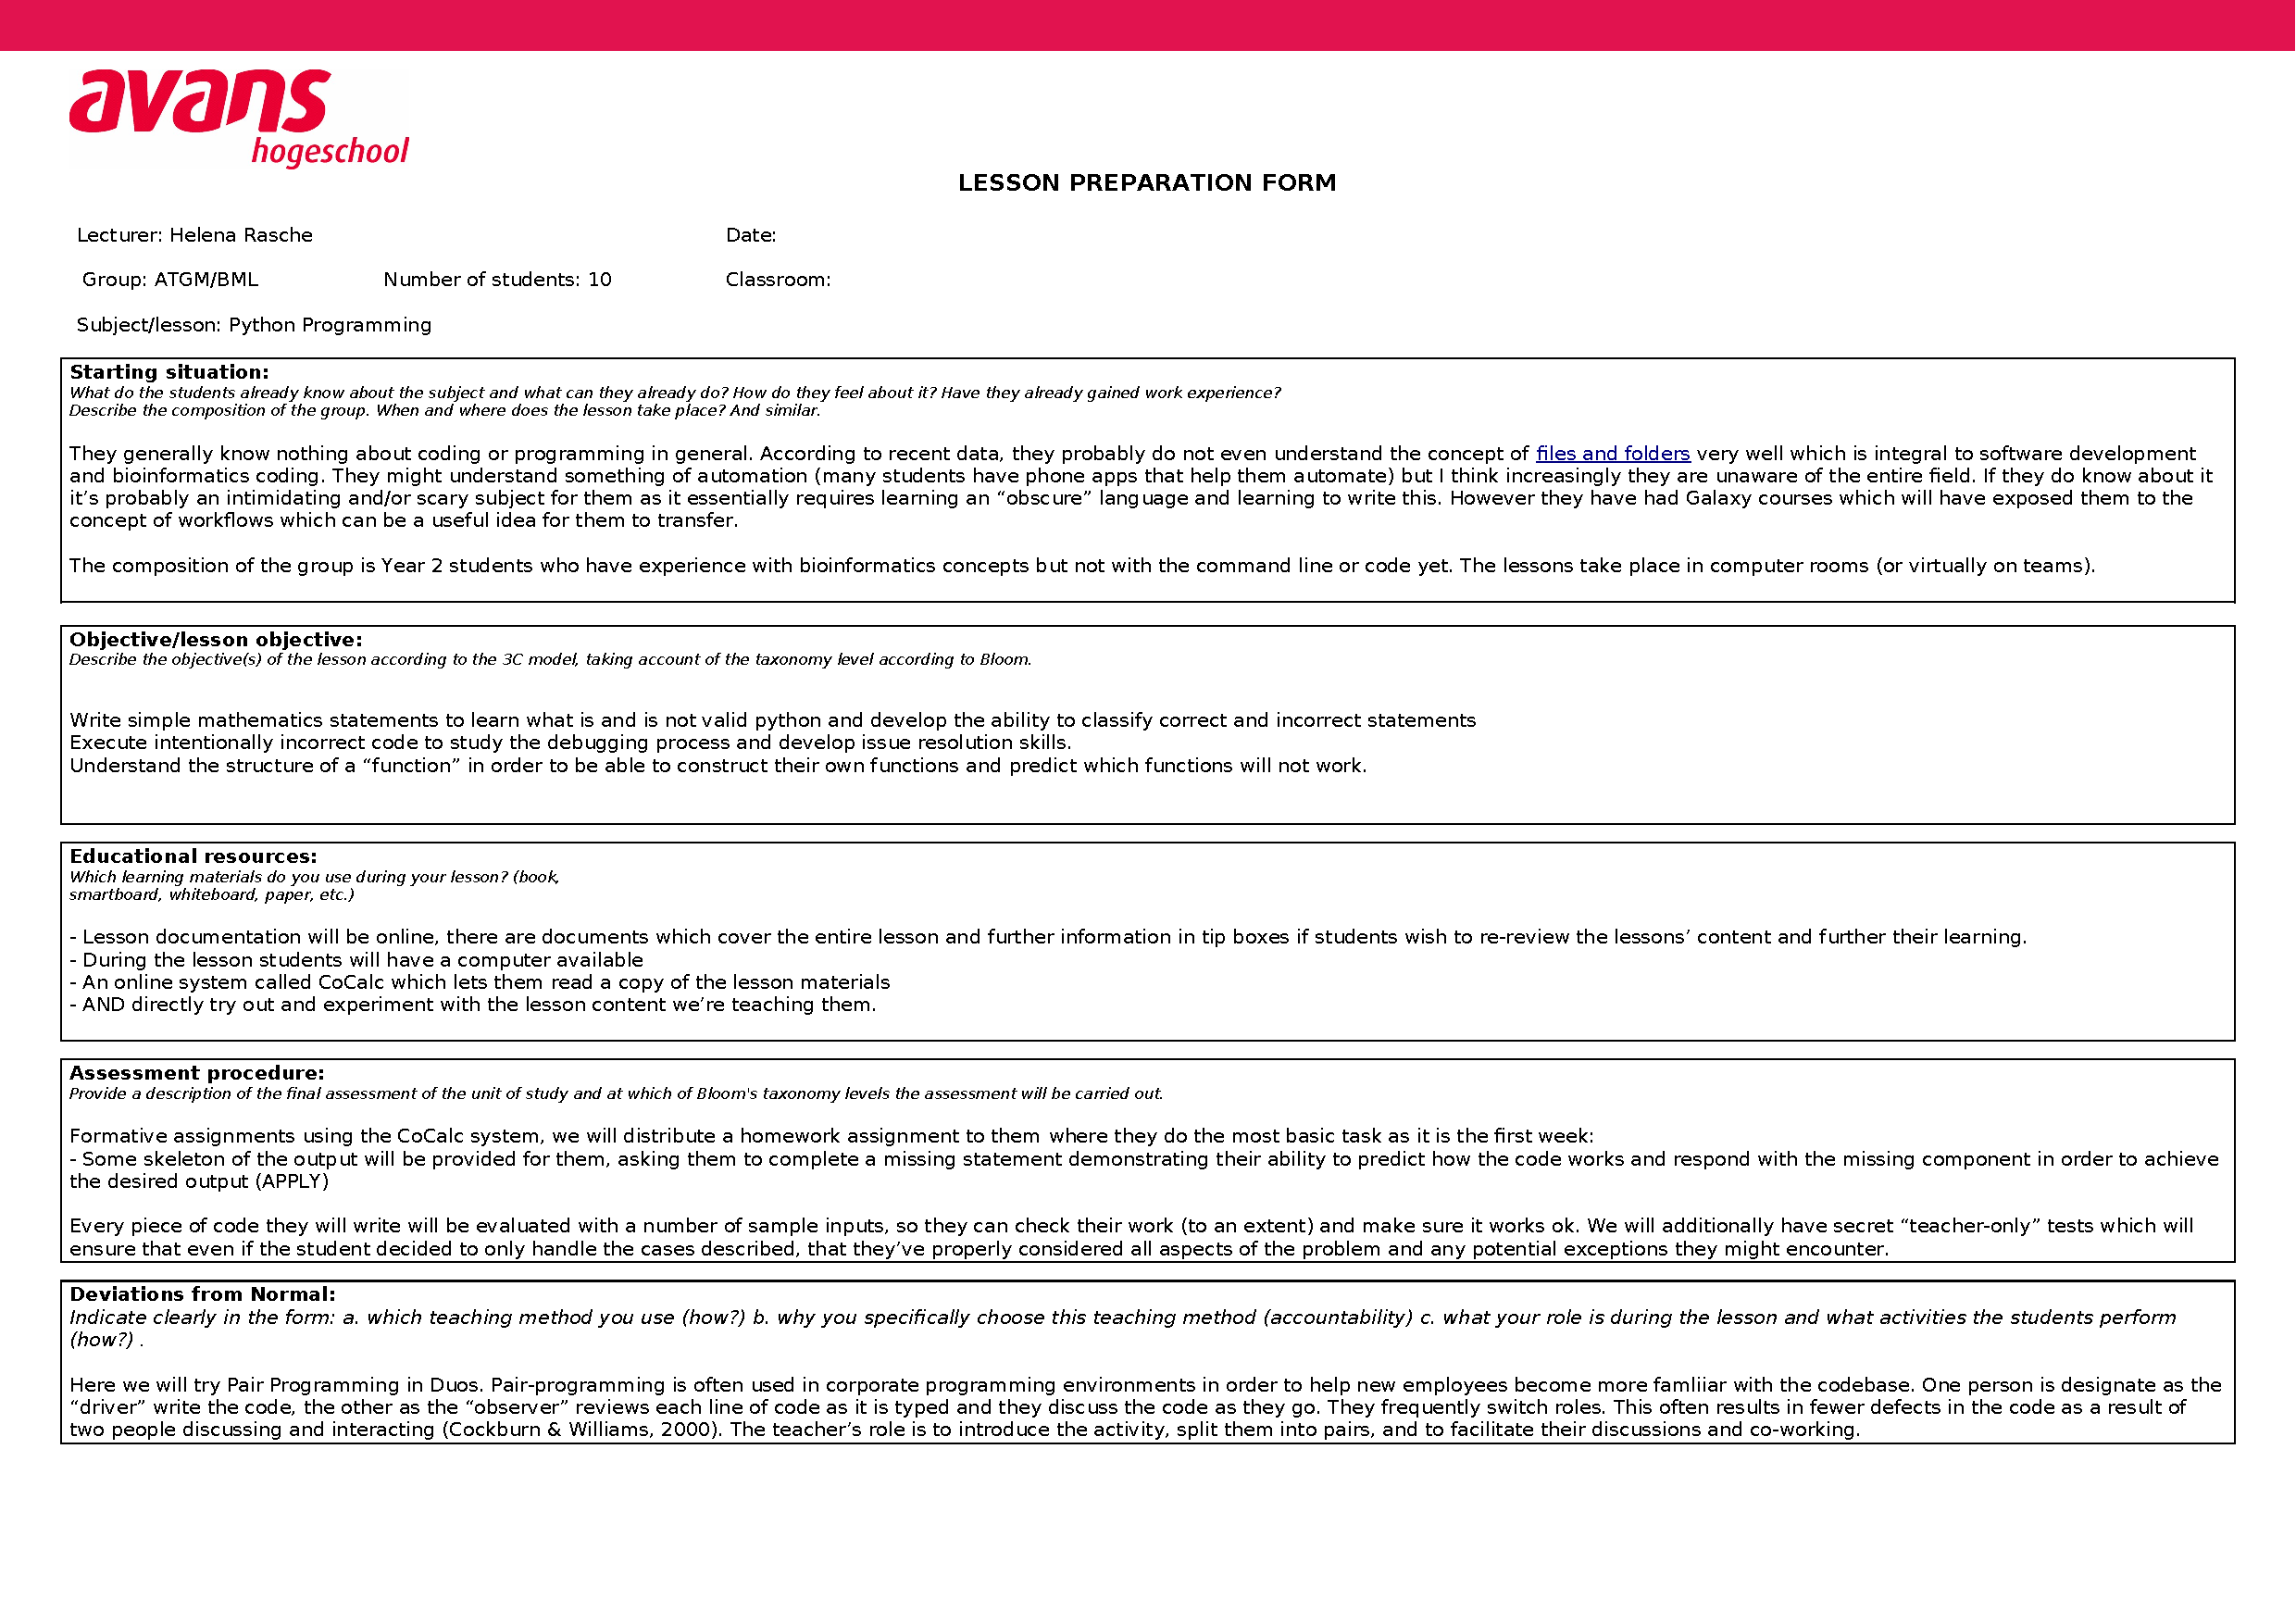
\includepdf[pages=-]{Lesson preparation form v2.pdf}

\end{document}
